\chapter{Introducción específica} % Main chapter title

\label{Chapter2}

%----------------------------------------------------------------------------------------

Este capítulo tiene como objetivo presentar las técnicas y herramientas clave utilizadas en el 
desarrollo de este trabajo. Se analizan los enfoques fundamentales para el procesamiento de 
lenguaje natural, junto con los modelos, frameworks e infraestructura necesarios para 
construir un sistema de recuperación de información eficiente y escalable. Este recorrido 
técnico permite comprender los fundamentos sobre los que se apoya la solución implementada. 

%---------------------------------------------------------------------------------------
\section{Técnicas de procesamiento de lenguaje natural}

El procesamiento de lenguaje natural (NLP) es un área de la inteligencia artificial que les permite 
a las máquinas comprender e interpretar el lenguaje humano \citep{book:nlp}. Esto juega un papel esencial 
para que un chatbot interprete las consultas de los usuarios y localice la información relevante en los 
documentos procesados. Las técnicas de NLP aplicadas contribuyen a que el sistema entienda el 
significado de las solicitudes, independientemente de variaciones lingüísticas o de sintaxis. Entre los 
métodos de mayor importancia para este trabajo se encuentran los \textit{word embeddings} y los
\textit{transformers}.

\subsection{\textit{Word embeddings}}

Los \textit{embeddings} son una poderosa técnica para transformar datos complejos en formas numéricas que 
son fácilmente procesadas y analizadas por algoritmos de aprendizaje automático \citep{paper:embeddings}. Esta técnica permite 
representar virtualmente cualquier tipo de dato como vectores, lo que posibilita su manipulación en tareas de 
procesamiento de lenguaje natural.

Sin embargo, no se trata solo de convertir las palabras en vectores. Es crucial preservar el significado original 
de los datos para que las tareas realizadas en este espacio transformado mantengan la coherencia semántica. 
Por ejemplo, al comparar dos frases, no solo se desea analizar las palabras que contienen, sino también evaluar 
si ambas expresan un significado similar.

Para conservar el significado, es necesario generar vectores donde las relaciones entre ellos sean representativas 
del contenido. Para ello, se emplea un modelo de \textit{embeddings} pre-entrenado, que produce una representación compacta 
de los datos mientras mantiene sus características semánticas. El objetivo es capturar el significado o las relaciones 
semánticas entre los puntos de datos, de modo que los elementos similares se encuentren cercanos en el espacio vectorial y los disímiles estén alejados. 
Por ejemplo, considerando las palabras ``rey'' y ``reina'', un \textit{embedding} podría mapear estas palabras en vectores de modo 
que la diferencia entre ``rey' y ``reina'' sea similar a la diferencia entre ``hombre'' y ``mujer'', y reflejar así las 
relaciones semánticas subyacentes.

En este trabajo, se ensayaron diferentes modelos de \textit{embeddings} de OpenAI, Google y Hugging Face, 
cuya evaluación y selección se detallan en el capítulo \ref{Chapter4}.

\subsection{Transformers}

La arquitectura de \textit{transformers} ha revolucionado el procesamiento de lenguaje natural al introducir un mecanismo de \textit{self-attention}, 
que permite a un modelo evaluar la relevancia de cada palabra en una secuencia en relación con las demás \citep{paper:transformers}. Este enfoque 
supera las limitaciones de modelos secuenciales tradicionales, ya que es capaz de procesar palabras en paralelo y captar dependencias de largo alcance 
en el texto. En lugar de analizar cada palabra en un orden específico, el mecanismo de \textit{self-attention} permite que el modelo ``preste atención'' 
a las palabras más relevantes en el contexto de la frase, al asignar pesos a cada una según su importancia relativa en la oración. Gracias a esta capacidad, 
los \textit{transformers} pueden capturar relaciones contextuales complejas y matices semánticos entre las palabras, 
lo que resulta fundamental para tareas como la generación de texto. Esta arquitectura ha hecho posible que los modelos comprendan y generen 
lenguaje natural de una forma mucho más cercana a la comprensión humana. Esta técnica 
ha sido fundamental en el desarrollo de los modelos grandes de lenguaje, que se introducen a continuación.

%----------------------------------------------------------------------------------------
\section{Modelos grandes de lenguaje}

Los modelos grandes de lenguaje (LLM, por su sigla en inglés) son redes neuronales de gran escala, entrenadas 
para comprender y generar texto en lenguaje natural. Estos modelos, basados en arquitecturas de \textit{transformers}, 
están compuestos por millones o incluso billones de parámetros, lo que les permite capturar patrones complejos y 
relaciones contextuales en vastos conjuntos de datos de texto. Los LLM son capaces de realizar múltiples 
tareas de procesamiento de lenguaje natural, como la generación de texto, la traducción 
automática y el resumen de documentos. En la tabla \ref{tab:llms} se presentan 
algunos de los modelos más relevantes en la actualidad \citep{website:lifearchitect}.

\vspace{5mm}

\begin{table}[h]
	\centering
	\caption[Modelos LLM disponibles en el mercado]{Modelos LLM disponibles en el mercado}
	\begin{tabular}{l c c c}    
		\toprule
		\textbf{Modelo} 	 & \textbf{Creador} 	& \textbf{Año de publicación}  & \textbf{Cant. de parámetros (aprox.)}\\
		\midrule
		GPT-4o               & OpenAI 				& 2024                         & 200 mil millones\\		
		Gemini 1.5      	 & Google				& 2024                         & 1,5 billones\\
		LLaMa 3         	 & Meta				    & 2024                         & 70 mil millones\\
        GPT-4         	     & OpenAI				& 2023                         & 1,76 billones\\
        LLaMa 2         	 & Meta				    & 2023                         & 70 mil millones\\
        Mistral-7B         	 & Mistral AI		    & 2023                         & 7 mil millones\\
        BLOOM         	     & BigScience		    & 2022                         & 176 mil millones\\
        GPT-3.5         	 & OpenAI				& 2022                         & 20 mil millones\\
		\bottomrule
		\hline
	\end{tabular}
	\label{tab:llms}
\end{table}

\vspace{5mm}

En este trabajo, el modelo LLM desempeña un papel central ya que es el encargado de entender las consultas de 
los usuarios y generar respuestas coherentes. Para seleccionar el modelo más adecuado, 
se ensayaron diferentes variantes, cuyos detalles se describen en el capítulo \ref{Chapter4}.

\subsection{Modelos LLM versus modelos tradicionales}

A continuación se mencionan las principales diferencias entre los modelos grandes de lenguaje y los
modelos tradicionales:

\begin{itemize}
	\item Los LLM pueden adaptarse a nuevas tareas simplemente utilizando ejemplos en el \textit{prompt}, 
	sin necesidad de modificar sus parámetros o re-entrenar. Esto contrasta con los modelos tradicionales, 
	que requieren grandes conjuntos de datos etiquetados y re-entrenarse cada vez que se incorporan nuevas tareas.
	\item Comprenden instrucciones en lenguaje natural, lo que les permite seguir indicaciones complejas e 
	incluso inferir reglas implícitas a partir de ejemplos. Los modelos tradicionales, en cambio, suelen necesitar 
	formatos de entrada específicos y siguen reglas programadas explícitamente, sin capacidad para inferir patrones 
	nuevos en tiempo real.
	\item Mantienen la coherencia en conversaciones largas y son capaces de recordar información dada en 
	partes previas del diálogo. Los modelos tradicionales procesan cada entrada de manera independiente y no pueden 
	conservar el estado conversacional.
	\item Permiten una interacción bidireccional, donde pueden solicitar aclaraciones y ajustar sus respuestas 
	en función del \textit{feedback} recibido. Los modelos tradicionales, en cambio, ofrecen una interacción unidireccional
	y no manejan \textit{feedback} en tiempo real.
	\item Un solo LLM es capaz de realizar múltiples tareas sin configuración adicional y de adaptar su salida según 
	el contexto. Por el contrario, los modelos tradicionales están diseñados para una tarea específica, por lo que 
	se requiere un modelo separado para cada tarea.
\end{itemize}

%----------------------------------------------------------------------------------------
\section{Generación aumentada por recuperación}

Una limitación importante que presentan los LLM es que, debido a su naturaleza generalista, pueden 
carecer de precisión cuando se aplican a dominios específicos, ya que su conocimiento está limitado a la información 
con la que fueron entrenados. Si bien esta información es sumamente vasta, no alcanza a cubrir la infinidad de temas 
posibles, y no contempla contenido no disponible en fuentes públicas.

Para abordar esta limitación, los LLM pueden adaptarse mediante la técnica conocida como recuperación aumentada por 
generación (RAG) \citep{paper:rag-1}, que integra fuentes de datos especializadas que mejoran su precisión 
en contextos concretos, como el entorno empresarial. De esta manera, los LLM pueden aprovechar su capacidad de 
comprensión profunda del lenguaje, pero también acceder a información precisa y actualizada de documentos específicos.

Básicamente, esta técnica consta de dos fases principales: primero, se realiza una búsqueda entre los documentos
provistos y se seleccionan fragmentos que sean relevantes para la consulta del usuario. Luego, un modelo LLM
utiliza esa información para construir una respuesta contextualizada. En la figura \ref{fig:rag} se ilustra
un diagrama básico de su funcionamiento.

\vspace{3mm}

\begin{figure}[ht]
	\centering
	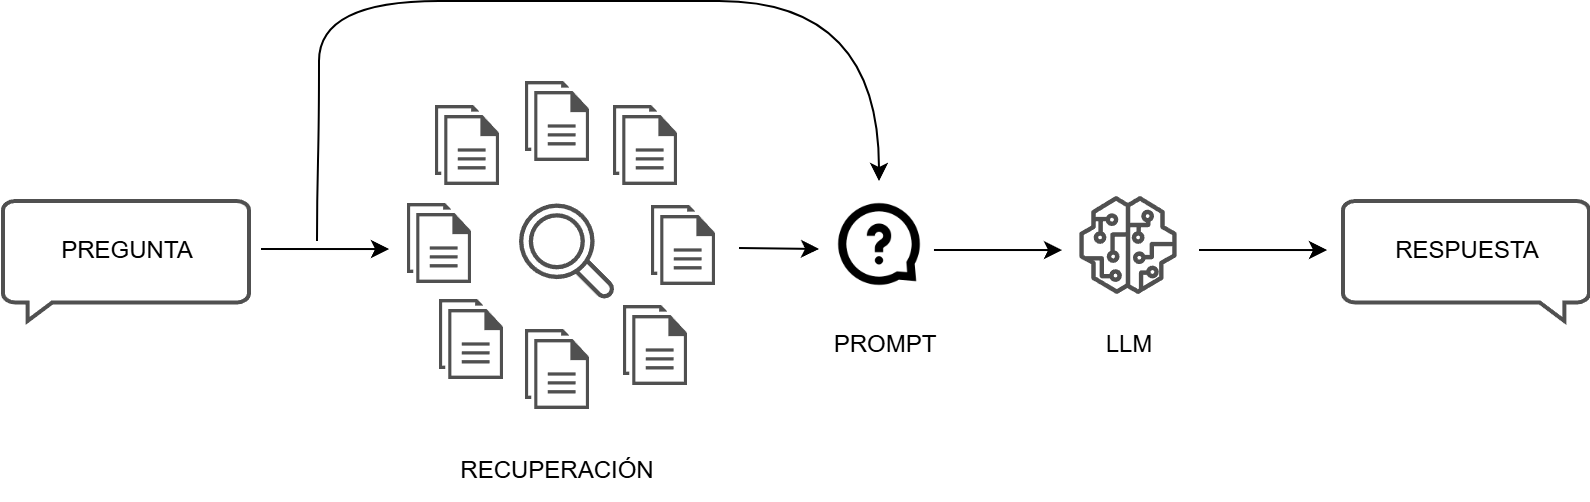
\includegraphics[scale=.24]{./Figures/rag.png}
	\caption{Diagrama de un sistema RAG.}
	\label{fig:rag}
\end{figure}

La combinación de recuperación y generación permite un flujo de información enriquecido, al lograr un equilibrio 
entre las capacidades generales del modelo y la especificidad requerida en el contexto empresarial.

%----------------------------------------------------------------------------------------
\section{Bases de datos vectoriales}

Una base de datos de vectorial \citep{article:vector-db} es una base de datos diseñada para almacenar y gestionar \textit{embeddings}. Esta
cumple un papel fundamental en la etapa de recuperación de información.

A diferencia de las bases de datos tradicionales, en las que las consultas suelen coincidir exactamente con los valores almacenados, 
las bases de datos vectoriales aplican métricas de similitud para identificar el vector más cercano a la consulta. 
El proceso de recuperación se realiza calculando la distancia entre 
el vector de la consulta y los vectores almacenados en la base de datos. Los fragmentos con menor distancia al vector 
de la consulta son seleccionados como los más relevantes y luego utilizados como insumo en la fase de generación de la respuesta. 

Para seleccionar la base de datos vectorial más adecuada para este trabajo, se exploraron varias opciones 
disponibles en el mercado, evaluando aspectos como el rendimiento y la facilidad de integración con el chatbot. 
Los resultados de estos ensayos se describen en el capítulo \ref{Chapter4}.

%----------------------------------------------------------------------------------------
\section{Frameworks utilizados}

En el desarrollo de este trabajo se utilizaron una serie frameworks que facilitaron la implementación de 
cada parte del sistema. A continuación, se detallan sus principales características y su rol específico en el producto final.

\begin{itemize}
	\item LangChain: este framework fue fundamental para la construcción del sistema RAG, ya que permite una gestión 
	eficiente de flujos de trabajo con modelos de lenguaje. LangChain facilita la integración de modelos LLM con fuentes de datos externas, 
	y además ofrece herramientas para diseñar flujos complejos 
	que manejan las consultas del usuario, el proceso de recuperación y la generación de respuestas \citep{website:langchain}.
	\item FastAPI: se utilizó para construir la API que conecta los componentes del sistema y gestiona las solicitudes del usuario. 
	Este framework, reconocido por su alto rendimiento y facilidad de uso, permitió desarrollar una API eficiente y escalable que procesa 
	las consultas en tiempo real. FastAPI facilita el manejo de solicitudes asíncronas y permite definir de manera clara los puntos 
	de conexión de la API, asegurando que las interacciones entre el frontend y el backend se 
	realicen de forma fluida y rápida \citep{website:fastapi}.
	\item NextUI: es un framework de diseño de interfaces de usuario 
	basado en React que permite construir interfaces modernas y responsivas. NextUI facilitó la creación de una interfaz intuitiva 
	y fácil de usar, que permite a los usuarios interactuar con el chatbot de manera fluida. Este framework ofrece una variedad de 
	componentes pre-construidos y altamente personalizables, lo que ayudó a reducir el tiempo de desarrollo de la interfaz y asegurar 
	una experiencia de usuario satisfactoria \citep{website:nextui}.
\end{itemize}

%----------------------------------------------------------------------------------------
\section{Servicios en la nube utilizados}

En este trabajo se empleó Microsoft Azure \citep{website:azure} como la plataforma principal de infraestructura en la nube, seleccionada por su robustez y 
variedad de servicios orientados a aplicaciones de inteligencia artificial. Azure ofrece soluciones 
escalables y seguras para gestionar datos y modelos, lo que facilita la integración de distintos recursos en un entorno controlado y eficiente.

Los recursos específicos de Azure utilizados incluyen:

\begin{itemize}
	\item Azure OpenAI: este recurso se utilizó para desplegar el modelo de lenguaje LLM y el modelo de \textit{embeddings}, 
	lo que provee la capacidad de procesamiento de lenguaje natural avanzada requerida por el sistema \citep{website:azure-openai}.
	\item Azure AI Search: utilizado como base de datos vectorial, este servicio permite almacenar y recuperar \textit{embeddings} 
	mediante búsquedas de similitud \citep{website:ai-search}.
	\item Azure App Service: empleado para hospedar el backend del chatbot, este servicio garantiza un entorno seguro y 
	escalable para la ejecución de la API y la gestión de consultas de los usuarios \citep{website:app-service}.
	\item Azure Static Web Apps: utilizado para hospedar el frontend del chatbot, proporciona un despliegue 
	rápido y eficiente de la interfaz de usuario y puede ser accedido por los empleados desde cualquier ubicación \citep{website:static-web-app}.
\end{itemize}

Además, se implementó GitHub Actions \citep{website:github-actions} como \textit{pipeline} de integración y despliegue continuo, no solo para publicar 
actualizaciones del backend y el frontend, sino también para automatizar la actualización del contenido de la base de datos.